\begin{center}
        \Large\textit{"Any sufficiently advanced technology is indistinguishable from magic."} -- Arthur C. Clarke
\end{center}

\section{Intelligenza Artificiale: Perché?}    
    Nonostante talvolta possa effettivamente sembrare magia, soprattutto quando prendiamo in considerazione tecnologie moderne come reti neurali e machine learning, e strumenti come assistenti vocali e Google Maps, l'intelligenza artificiale, alla base, altro non è che una specifica tipologia di algoritmi, seppur con una particolare filosofia dietro.
    
    Il motivo per cui oggi è così pervasiva e per cui così tanti investimenti vanno nei suoi confronti è che è capace di risolvere problemi altresì molto complessi, e talvolta sostituire gli umani in alcuni compiti. Tuttavia questi algoritmi non sono autonomi, e hanno comunque bisogno di un buon progettista per funzionare a dovere. Possiamo motivare l'hype dietro questa tecnologia con cinque punti:
    
    \begin{enumerate}
        \item Ottimizzazione di risorse.
        \item Necessità di velocizzare l'apprendimento nell'esecuzione di task.
        \item Risoluzione di problemi umanamente complessi.
        \item Marketing.
        \item Curiosità.
    \end{enumerate}
    
    \subsection{Obiettivi di apprendimento}
        Questo corso si divide in due macroargomenti, che hanno tuttavia alla base il semplice concetto di \textbf{agente intelligente}.
        
        I due macroargomenti e i loro relativi sottoargomenti sono:
        
        \begin{itemize}
            \item Risoluzione di problemi con la ricerca:
            \begin{itemize}
                \item Strategie di ricerca informata e non-informata.
                \item Ricerca locale, ottimizzazione.
                \item Ricerca con avversari.
            \end{itemize}
            \item Risoluzione di problemi tramite l'apprendimento:
            \begin{itemize}
                \item Teoria dell'apprendimento.
                \item Apprendimento supervisionato.
                \item Apprendimento non supervisionato.
            \end{itemize}
        \end{itemize}
        
\section{Definizione di Intelligenza Artificiale}
    Per migliaia di anni siamo stati, come specie umana, affascinati dalla nostra stessa intelligenza e abbiamo cercato di comprenderla.
    
    L'intelligenza artificiale fa un ulteriore passo e cerca di \textbf{costruire} entità intelligenti.

    La definizione di Intelligenza Artificiale non è banale, e infatti ce ne sono diverse e composte da vari aspetti. Noi definiamo \textbf{quattro} caratteristiche che un Agente deve avere per essere definito Intelligente.
        
    \begin{enumerate}
        \item \textbf{Pensare umanamente.} Far sì che i computer pensino ed eseguono attività comunemente associate al pensiero umano come l'apprendimento, il processo decisionale, etc.
        \item \textbf{Pensare razionalmente.} Lo studio dei processi di calcolo che rendono possibile percepire, ragionare, etc.
        \item \textbf{Agire umanamente.} L'arte di creare macchine che eseguono azioni che, quando eseguite da esseri umani, richiedono intelligenza, o comunque a cui, al momento, le persone sono più brave.
        \item \textbf{Agire razionalmente.} Forse aspetto più importante, riguarda un comportamento intelligente e dotato di criterio.
    \end{enumerate}
        
    Andiamo a vedere più nello specifico i vari aspetti.
    
    \subsection{Pensare umanamente}
        Quando diciamo che un determinato programma ragiona come un essere umano, dobbiamo innanzitutto determinare come noi pensiamo, e capire cioè i meccanismi interni del cervello umano. Abbiamo tre modi per modellare questi meccanismi interni:
        \begin{itemize}
            \item \textbf{Introspezione.} Atto della coscienza che consiste nell'osservazione diretta e nell'analisi dell'interiorità rappresentata da pensieri, pulsioni, desideri etc. La modellazione, in questo caso, consiste nel catturare "al volo" i nostri pensieri mentre scorrono.
            \item \textbf{Sperimentazione psicologica.} È la branca della psicologia che tenta di applicare il metodo sperimentale all'indagine dei processi cognitivi del cervello. La modellazione in questo caso consiste nell'osservazione di pensieri, pulsioni, stimoli etc. di una persona in azione.
            \item \textbf{Imaging celebrale.} Consiste nella mappatura, diretta o indiretta, della struttura e delle funzioni del sistema nervoso. La modellazione in questo caso consiste nell'osservazione del cervello in azione, così da poterne intuire i meccanismi nervosi interni e trarne conclusioni.
        \end{itemize}
        
        C'è ora da specificare l'importanza, all'interno dello studio dell'intelligenza artificiale, della \textbf{psicologia} e delle \textbf{neuroscienze}: la prima si chiede come agiscono e pensano esseri umani ed animali, mentre le neuroscienze si pongono domande sui meccanismi che permettono l'elaborazione di informazioni da parte del cervello.
        
        Secondo Craik, un Agente Intelligente possiede tre requisiti fondamentali:
        \begin{enumerate}
            \item Lo stimolo esterno deve essere tradotto in una rappresentazione interna.
            \item Tale rappresentazione interna deve essere manipolata da processi cognitivi per ottenere nuove rappresentazioni interne.
            \item Tali nuove rappresentazioni devono a loro volta essere trasformate in azioni.
        \end{enumerate}
        
        \begin{center}
            \large\textit{“Se l’organismo porta nella sua testa un ‘modello in scala’
                della realtà esterna e delle proprie possibili azioni sarà in
                grado di provare varie alternative, decidere quali di esse sia
                la migliore, reagire a situazioni future prima che si
                manifestino, utilizzare la conoscenza di eventi passati per
                gestire quelli presenti e futuri, e sotto ogni aspetto reagire in
                modo molto più ricco, affidabile e competente alle
                emergenze che si troverà a fronteggiare.”} -- K. J. W. Craik
            \end{center}
            
            Questa è probabilmente la miglior definizione di Intelligenza Artificiale che mai avremo, nonostante sia stata formulata quasi un secolo fa.
            
            Un altro importante contributo di Craik fu quello di fondare le scienze cognitive, che ad oggi ci danno importanti indizi sul funzionamento del sistema nervoso e in particolare del cervello. Sappiamo che alla base del pensiero ci sono i neuroni, che comunicano fra loro tramite punti di congiunzione detti sinapsi, e che oltre a collegamenti immediati possono anche cambiare permanentemente la loro struttura, dando così quella che ad oggi riteniamo essere la base dell'apprendimento.
            
            Un'altra importante nozione è la potenza del cervello. Con le conoscenze odierne sappiamo che, nonostante gli enormi progressi tecnologici che abbiamo fatto, un cervello umano ha una capacità di memorizzazione e velocità di computazione maggiore rispetto agli odierni supercomputer. Ovviamente il raggiungimento di questa soglia non vuol dire automaticamente la nascita della coscienza artificiale, in quanto è inutile per un computer eseguire $10^{17}$ operazioni al secondo se queste operazioni non sono ben finalizzate allo scopo di pensare e agire razionalmente.
         
        \newpage   
    \subsection{Pensare razionalmente}
        Pensare razionalmente vuol dire usare in maniera corretta la logica. Si ritiene che suddetta disciplina abbia avuto origine con i \textbf{sillogismi aristotelici}, ossia i primi tentativi di codificare formalmente il pensiero corretto.
            
        Questo col tempo è sfociato nel logicismo. Questa disciplina sostiene che è necessario partire da enunciati logici per costruire sistemi intelligenti e razionali. Tuttavia sorgono due importanti problemi:
        \begin{enumerate}
            \item Non è facile esprimere una conoscenza non formale (ossia il mondo reale, dominato anche da un certo grado di caos e soggettività) in termini formali.
           \item Ancora più importante, è diverso definire un enunciato in maniera logica ed agire in maniera da soddisfare quella condizione. Per esempio leggere un buon libro riguardante l'Intelligenza Artificiale non equivale automaticamente al superamento del relativo esame.
        \end{enumerate}
            
        Con un approccio del genere, anche problemi con poche centinaia di variabili possono risultare impossibili da risolvere, in quanto potrebbero saturare completamente le risorse computazionali disponibili. Abbiamo pertanto bisogno di una maniera per navigare queste infinite possibilità senza necessariamente esplorarle tutte. Questa rappresenta una sfida aperta nel campo dell'Intelligenza Artificiale.
        
    \subsection{Agire Umanamente}
        Un modo per verificare l'agire umano di una macchina potrebbe essere il test di Turing, conosciuto anche come the Imitation Game.
        
        Turing ebbe numerose critiche, di natura più o meno sensata, durante la sua vita riguardo questo test.
        
        Al contrario di molte critiche di natura filosofica e regligiosa, una limitazione piuttosto concreta venne proposta da Kurt Gödel. È proprio il \textbf{teorema di Gödel} a dimostrare che in qualsiasi sistema logico sufficientemente potente si possono formulare proposizioni che non è possibile provare nè tantomeno smentire, all'interno del sistema, derivando così una possibilità di incoerenza all'interno dello stesso sistema logico.
        
        Lo stesso Turing ottenne risultati simili. Tuttavia, vale la pena sottolineare che le stesse limitazioni sottolineate dal teorema di Gödel potrebbero valere anche per l'intelletto umano. Non esiste, ad oggi, nessuna dimostrazione a proposito.
        
    \subsection{Agire Razionalmente}
        Questo è forse il più importante dei quattro punti. Un agente per essere tale deve fare qualcosa, e quindi gli algoritmi, per definizione, sono agenti. Da un Agente Intelligente tuttavia si richiede qualcosa in più, ossia che egli sia capace di agire autonomamente, imparare dal passato per migliorare nel futuro.
        
        Un agente razionale agisce in maniera da ottenere il miglior risultato possibile, ma che in situazioni di incertezza riesce comunque a prendere una decisione in base al miglior risultato atteso basandosi sulle sue conoscenze pregresse.
        
        Quest'ultimo punto in particolare va in contrasto con la logica classica in quanto prende in considerazione un certo grado di caos e approssimazione. L'agire razionalmente \textbf{include} i tre punti precedenti nonché l'idea aggiuntiva di adattarsi al contesto, facendo la scelta migliore fra le disponibili basandosi sulla conoscenza pregressa.
        
\section{Agenti Intelligenti}
    Un \textbf{agente} è qualsiasi cosa possa essere vista come un sistema che \textit{percepisce} l'ambiente in cui si trova tramite dei \textbf{sensori} ed \textit{agisce} su di esso tramite degli \textbf{attuatori}.
    
    \begin{figure}[h]
        \centering
        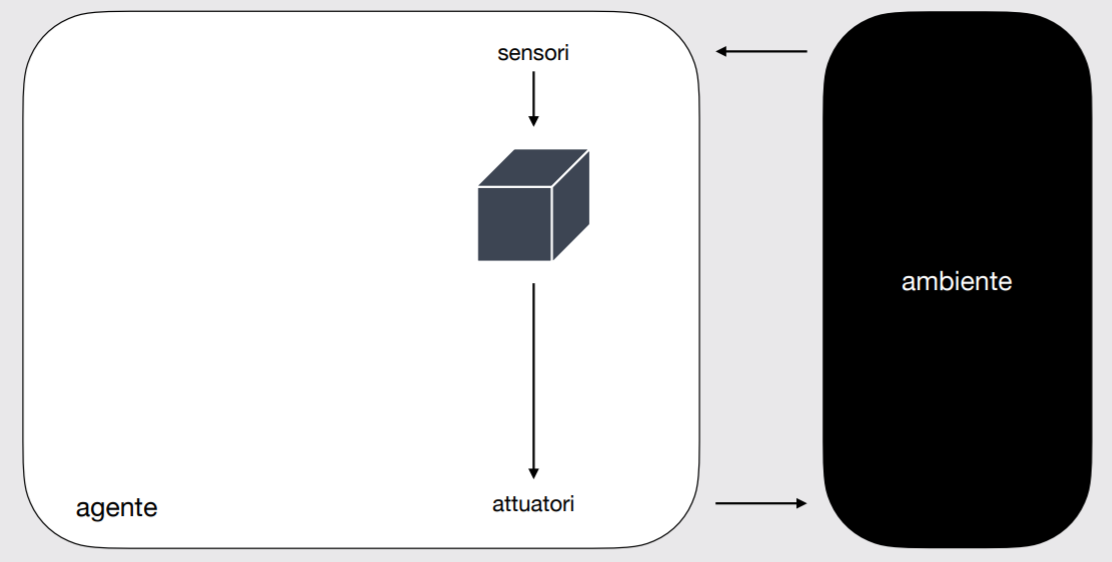
\includegraphics[width=0.90\textwidth]{img/img1.png}
        \caption{Rappresentazione di un agente relativamente all'ambiente in cui si trova.}
        \label{fig:un_agente}
    \end{figure}
    
    \subsection{Come si comporta un Agente Intelligente}
    
        Due importanti \textbf{definizioni} che ci servono per capire cosa è un agente intelligente e come si comporta:
        \begin{enumerate}
            \item \textbf{Percezione:} Insieme degli input percettivi in un dato istante.
            \item \textbf{Sequenza percettiva:} Storia completa di tutto ciò che l'agente ha percepito nella sua esistenza.
        \end{enumerate}
        
        La scelta di un'azione da parte di un agente può essere determinata da ciò che ha percepito (ma non necessariamente lo sarà) ma sicuramente non può essere determinata da ciò che non ha percepito. Questa è un'importante differenza fra un umano e un agente software, in quanto l'umano può comportarsi in modo imprevedibile, facendo cose non necessariamente collegate allo storico delle sue percezioni (pensiamo a una persona che agisce da ubriaca).
        
        Se volessimo dirla in termini prettamente matematici, allora il comportamento di un agente è descritto da una \textbf{funzione agente}, che descrive la corrispondenza fra una qualsiasi sequenza percettiva e una specifica azione. Da un punto di vista pratico la funzione agente è implementata tramite uno specifico \textbf{programma agente}.
        
        Questa relazione potrebbe essere per esempio espressa tramite una tabella. Riusciamo con non troppe difficoltà a intuire che anche con pochi parametri, questa tabella potrebbe raggiungere dimensioni difficili da gestire. Quindi dobbiamo capire come generarla, come esplorarla, ossia cosa rende un agente buono, cattivo, intelligente o stupido.
        
    \subsection{Valutare un Agente Intelligente}
        La razionalità di un agente dipende dalla sue \textbf{prestazioni}, dalla sua \textbf{conoscenza pregressa}, dalle \textbf{azioni che può compiere} e dalla \textbf{sequenza percettiva fino all'istante corrente}. Proprio come accade per un essere umano, la razionalità dipende da quanto è razionale in base alle sue conoscenze, in base al suo obiettivo e tenendo in considerazione l'ambiente che lo circonda, quindi queste quattro caratteristiche non vanno viste in maniera isolata ma va considerato come interagiscono fra loro.
        
        Per ogni possibile sequenza di percezioni, un agente razionale dovrebbe scegliere un'azione che massimizzi il valore atteso della sua \textit{misura di prestazione}, date tutte le informazioni che ha, sia quelle fornite dalla sequenza percettiva che non.
        
        La suddetta \textbf{misura di prestazione} dovrebbe essere progettata in base all'effetto che si desidera osservare sull'ambiente, e non sul comportamento che ci si aspetta dall'agente. Il rischio in tal caso sarebbe di ottenere un agente che si "illude" di fare la cosa giusta senza verificare che il risconto nell'ambiente circostante sia positivo.
        
        \textbf{Attenzione}: la razionalità non implica l'\textbf{onniscienza}. Un agente onnisciente conosce il risultato di ogni singola sua azione e può agire di conseguenza, ma nella realtà l'onniscenza raramente è ottenibile. Un agente \textbf{razionale} invece prova a fare la cosa "giusta" in base al contesto in cui si trova, avendo come obiettivo la massimizzazione del risultato atteso.
        
        \paragraph{Information Gathering.} Talvolta è opportuno e ottimale eseguire azioni cosiddette di information gathering, le quali hanno il solo scopo di conoscere l'ambiente circostante, e che consentono di rendere più efficaci le azioni future. Una tale azione in un essere umano potrebbe essere il guardare a destra e sinistra prima di attraversare.
        
        Un secondo esempio di information gathering è detto \textbf{esplorazione}, necessaria a far conoscenza di un ambiente sconosciuto e che vedremo negli algoritmi di ricerca.
        
        \paragraph{Apprendimento} Un altro aspetto importante della razionalità è l'apprendimento, ossia la capacità di fare nuove associazioni di coppie percezione-azione in base ai risultati visti in precedenza, oltre di modificare quelle già conosciute. Un agente che agisce in base alla conoscenza pregressa ma che non impara potrebbe anche essere efficace, ma mancherà di autonomia.
        
\section{Ambienti}
    Un \textbf{ambiente} è essenzialmente l'istanza di un problema di cui gli agenti razionali rappresentano le soluzioni.
    
    \subsection{Formulazione P.E.A.S.}
        Un ambiente viene generalmente descritto tramite la formulazione P.E.A.S.:
        \begin{enumerate}
            \item \textbf{P.} Misura di prestazione dell'operato di un agente.
            \item \textbf{E.} Descrizione degli elementi che formano l'ambiente.
            \item \textbf{A.} Gli attuatori disponibili all'agente per intraprendere azioni.
            \item \textbf{S.} I sensori attraverso i quali l'agente riceve gli input percettivi.
        \end{enumerate}
        
        \paragraph{Proprietà degli ambienti.} Possiamo identificare un numero relativamente piccolo di dimensioni per caratterizzare gli ambienti, andando di fatti a semplificare molto la loro enorme complessità e varietà nel mondo reale.
        \begin{itemize}
            \item \textbf{Completamente o parzialmente osservabili:} Un ambiente è completamente osservabile se i sensori di un agente hanno accesso al suo stato completo in ogni momento.
            \item \textbf{Deterministico o stocastico:} È deterministico se lo stato successivo è determinato unicamente dallo stato corrente e dall'azione intrapresa dall'agente.
            \item \textbf{Episodico o sequenziale:} È episodico se l'esperienza dell'agente è divisa in "episodi" atomici, dove ciascun episodio consiste nell'eseguire una singola azione.
            \item \textbf{Statico o dinamico:} È statico se non cambia mentre l'agente sta deliberando. Un ambiente si dice invece semi-dinamico se esso non cambia col tempo ma il punteggio di prestazione dell'agente sì.
            \item \textbf{Discreto o continuo:} È discreto se fornisce un numero limitato di percezioni e possibili azioni distinte, chiaramente definite. Il gioco degli scacchi è un ambiente discreto, mentre un'auto a guida autonoma è continuo.
            \item \textbf{Singolo o multi-agente:} È singolo quando prevede la presenza di un unico agente. Quando ve ne sono molteplici lo scenario cambia, e come vedremo in futuro i vari agenti potrebbero collaborare o comportarsi come avversari l'uno nei confronti dell'altro. In particolare:
            \begin{itemize}
                \item \textbf{Competitivo:} L'ambiente multi-agente si dice competitivo quando un agente mira a massimizzare/minimizzare la misura di prestazione dell'altro.
                \item \textbf{Cooperativo:} È invece cooperativo quando i vari agenti mirano a massimizzare/minimizzare la stessa misura di prestazione.
            \end{itemize}
        \end{itemize}
        
\section{Struttura degli agenti}
    Fin qui abbiamo visto gli agenti come delle \textit{black box}, descrivendo il loro comportamento in base alle percezioni ricevute. Volendo fare un passo verso la progettazione di un agente, e dando per scontata la sua esecuzione su un computer dotato di attuatori e sensori, che insieme costituiscono l'\textbf{architettura}, diremo che: \textit{agente = programma + architettura}.
    
    È importante la distinzione fra \textbf{programma} e \textbf{funzione} agente: il primo prende in input solo la percezione corrente, mentre il secondo tutta la storia percettiva. La sfida dell'intelligenza artificiale è scrivere programmi che, nella massima misura possibile, producano un comportamento razionale con una piccola quantità di codice, anziché rappresentare tutti i possibili input percettivi possibili. Proprio in funzione di ciò ci risulta impossibile generare tabelle per ogni possibile percezione. In un gioco relativamente semplice nella sua formulazione come quello degli scacchi avremmo una tabella di $10^{150}$ righe.
    
    Iniziamo a vedere dunque qualche alternativa più efficace. Tutti gli agenti che vedremo sono classificati come \textbf{learning agents}, ossia agenti capaci di migliorare le loro prestazioni e attuare azioni migliori tramite l'apprendimento.
    
\section{Agenti davvero intelligenti}
    \subsection{Agenti reattivi semplici}
        Questi semplicissimi agenti intraprendono un'azione in base alla percezione appena ricevuta, ignorando la storia pregressa. Pertanto, non hanno memoria.
        
        Il vantaggio è l'estrema semplicità dell'implementazione, spesso effettuata con un semplice \texttt{if-then}. Per problemi che non necessariamente richiedono una grande conoscenza delle percezioni pregresse, questa soluzione potrebbe essere un buon compromesso.
        
        Questo tipo di agente funziona solo in caso di ambienti completamente osservabili. In caso di informazioni mancanti potrebbe incappare in \textbf{cicli infiniti}. Una soluzione a questo problema è aggiungere una componente casuale la quale verrà invocata nel caso di dati mancanti. Come vedremo in futuro, una componente casuale porta spesso a un comportamento razionale. Questo non è il caso, in quanto la componente casuale serve solo a non incappare in suddetti cicli infiniti.
        
    \subsection{Agenti reattivi basati su Modello}
        Questo tipo di agenti ha due tipi di conoscenza: come evolve il mondo, indipendentemente dal suo stato; e informazioni riguardanti l'impatto delle sue azioni sull'ambiente.
        
        La conoscenza del mondo sviluppata tramite una teoria scientifica completa viene chiamata appunto \textbf{modello} del mondo.
        
        È importante considerare che lo stato attuale che l'agente considera non coincide necessariamente con lo stato del mondo (l'agente non è onnisciente), ma con la migliore ipotesi che l'agente può fare.
        
    \subsection{Agenti basati su Obiettivi}
        È un agente che aggiunge al modello informazioni sugli specifici obiettivi che si intende raggiungere. In pratica, conoscere lo stato del mondo non sempre è necessario ad arrivare in maniera rapida e precisa, quindi potrebbe convenire definire obiettivi verso i quali gli agenti si possono muovere. Questi obiettivi non coincidono con le coppie condizione-azione viste in precedenza, in quanto prendono in considerazione previsioni del cambiamento dell'ambiente in base all'azione compiuta, e non sono quindi necessariamente deterministici.
        
    \subsection{Agenti basati sull'utilità}
        Gli obiettivi consentono di esprimere condizioni "buone" e "cattive". Nella realtà tuttavia  potremmo avere vie di mezzo, come situazioni "desiderabili" o meno.
        
        Una funzione di utilità ci indica quanto un determinato obiettivo è desiderabile, associando un numero e non necessariamente un booleano a questo parametro. Potremmo avere più funzioni di utilità fra di loro contrastanti, e in questo caso l'agente deve prendere una decisione basandosi su delle priorità.
        
    \subsection{Agenti capaci di apprendere}
        L'apprendimento presenta il vantaggio di mettere agenti in ambienti inizialmente sconosciuti e permettergli di imparare e migliorare. Un agente di questo tipo ha quattro componenti principali:
        \begin{itemize}
            \item \textbf{Elemento di apprendimento:} L'elemento responsabile del miglioramento interno.
            \item \textbf{Elemento esecutivo:} L'elemento responsabile della selezione delle azioni esterne. Questo è ciò che fino ad ora abbiamo considerato come agente.
            \item \textbf{Elemento critico:} L'elemento responsabile di dare feedback sulle prestazioni correnti, così che l'elemento di apprendimento possa determinare se e come modificare l'elemento esecutivo in maniera che si comporti meglio in futuro.
            \item \textbf{Generatore di problemi:} L'elemento responsabile di suggerire all'agente azioni che portino ad esperienze nuove e significative, in particolare esperienze che possano favorire l'apprendimento.
        \end{itemize}